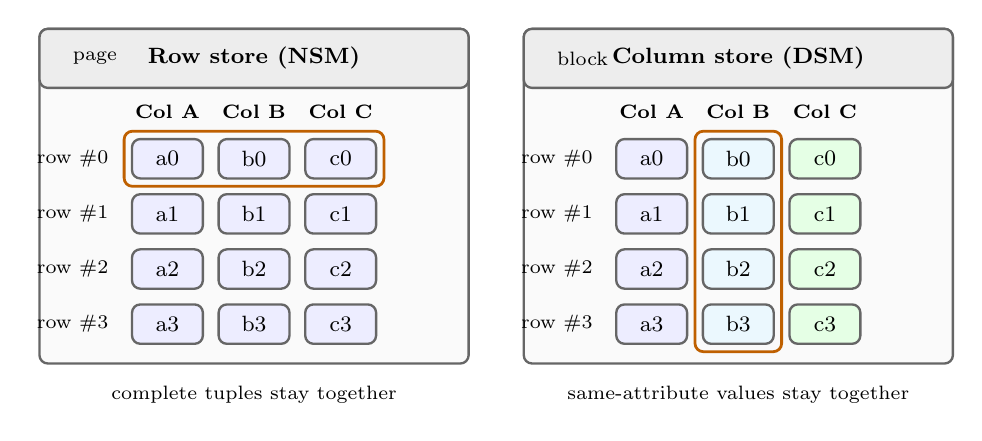
\begin{tikzpicture}[
    x=1cm,y=1cm,
    every node/.style={font=\footnotesize},
    frame/.style={draw=black!60, rounded corners=3pt, line width=0.85pt},
    header/.style={frame, fill=gray!14},
    cell/.style={frame, minimum width=0.90cm, minimum height=0.50cm, fill=blue!7},
    acol/.style={frame, minimum width=0.90cm, minimum height=0.50cm, fill=blue!7},
    bcol/.style={frame, minimum width=0.90cm, minimum height=0.50cm, fill=cyan!8},
    ccol/.style={frame, minimum width=0.90cm, minimum height=0.50cm, fill=green!10},
    accent/.style={draw=orange!75!black, rounded corners=3pt, line width=1.0pt}
]
    \draw[frame, fill=gray!4] (0,0) rectangle (5.45,4.25);
    \draw[header] (0,3.50) rectangle (5.45,4.25);
    \node[font=\footnotesize\bfseries] at (2.725,3.875) {Row store (NSM)};
    \node[font=\scriptsize, anchor=west] at (0.30,3.875) {page};

    \foreach \x/\lbl in {1.625/A, 2.725/B, 3.825/C} {
        \node[font=\scriptsize\bfseries] at (\x,3.20) {Col \lbl};
    }
    \foreach \r/\y in {0/2.60, 1/1.90, 2/1.20, 3/0.50} {
        \node[font=\scriptsize, anchor=east] at (1.00,\y) {row \#\r};
    }

    \node[cell] at (1.625,2.60) {a0};
    \node[cell] at (2.725,2.60) {b0};
    \node[cell] at (3.825,2.60) {c0};
    \node[cell] at (1.625,1.90) {a1};
    \node[cell] at (2.725,1.90) {b1};
    \node[cell] at (3.825,1.90) {c1};
    \node[cell] at (1.625,1.20) {a2};
    \node[cell] at (2.725,1.20) {b2};
    \node[cell] at (3.825,1.20) {c2};
    \node[cell] at (1.625,0.50) {a3};
    \node[cell] at (2.725,0.50) {b3};
    \node[cell] at (3.825,0.50) {c3};
    \draw[accent] (1.075,2.25) rectangle (4.375,2.95);

    \draw[frame, fill=gray!4] (6.15,0) rectangle (11.60,4.25);
    \draw[header] (6.15,3.50) rectangle (11.60,4.25);
    \node[font=\footnotesize\bfseries] at (8.875,3.875) {Column store (DSM)};
    \node[font=\scriptsize, anchor=west] at (6.45,3.875) {block};

    \foreach \x/\lbl in {7.775/A, 8.875/B, 9.975/C} {
        \node[font=\scriptsize\bfseries] at (\x,3.20) {Col \lbl};
    }
    \foreach \r/\y in {0/2.60, 1/1.90, 2/1.20, 3/0.50} {
        \node[font=\scriptsize, anchor=east] at (7.15,\y) {row \#\r};
    }

    \node[acol] at (7.775,2.60) {a0};
    \node[acol] at (7.775,1.90) {a1};
    \node[acol] at (7.775,1.20) {a2};
    \node[acol] at (7.775,0.50) {a3};

    \node[bcol] at (8.875,2.60) {b0};
    \node[bcol] at (8.875,1.90) {b1};
    \node[bcol] at (8.875,1.20) {b2};
    \node[bcol] at (8.875,0.50) {b3};

    \node[ccol] at (9.975,2.60) {c0};
    \node[ccol] at (9.975,1.90) {c1};
    \node[ccol] at (9.975,1.20) {c2};
    \node[ccol] at (9.975,0.50) {c3};
    \draw[accent] (8.325,0.15) rectangle (9.425,2.95);

    \node[font=\scriptsize] at (2.725,-0.40) {complete tuples stay together};
    \node[font=\scriptsize] at (8.875,-0.40) {same-attribute values stay together};
\end{tikzpicture}
